\documentclass[conference]{IEEEtran}
\hyphenation{OpenAi GPT-J}
\usepackage{svg}
\usepackage{float}
\usepackage{tikz}
\usepackage{makecell}
\usepackage{url}
\def\UrlBreaks{\do\/\do-}
\usepackage{breakurl}
\usepackage[breaklinks]{hyperref}
\usepackage{lipsum}  
\usepackage{listings}
\usepackage{xcolor}
\usepackage{setspace}
\usepackage{graphicx}
\usepackage{ragged2e}
\colorlet{punct}{red!60!black}
\definecolor{background}{HTML}{fafafa}
\definecolor{delim}{RGB}{20,105,176}
\colorlet{numb}{magenta!60!black}

\lstdefinelanguage{json}{
    basicstyle=\normalfont\ttfamily,
    numbers=left,
    numberstyle=\scriptsize,
    stepnumber=1,
    numbersep=8pt,
    showstringspaces=false,
    breaklines=true,
    frame=lines,
    backgroundcolor=\color{background},
    literate=
      {:}{{{\color{punct}{:}}}}{1}
      {,}{{{\color{punct}{,}}}}{1}
      {\{}{{{\color{delim}{\{}}}}{1}
      {\}}{{{\color{delim}{\}}}}}{1}
      {[}{{{\color{delim}{[}}}}{1}
      {]}{{{\color{delim}{]}}}}{1},
}


\begin{document}
\begin{titlepage}
    \centering
    \includegraphics[width=0.2\textwidth]{logoBlackV.eps}\par
    \vspace{1.5cm}
    {\LARGE Southern Adventist University \par}
    \vfill
    {\Large Senior Capstone Research Project\par}
    \vspace{1cm}
    {\huge\bfseries Evaluating the Performance of Large Transformer Networks Trading the News\par}
    \vspace{1cm}
    {\large Joel \textsc{Peckham}\par}
    \textsc{Email:} \href{mailto:joelskyler@gmail.com}{joelskyler@gmail.com}\par
    
    \vspace{0.5cm}
    supervised by\par
    Willard \textsc{Munger}, PhD.\par
    Robert \textsc{Ordóñez}, M.S.
    \vfill
    \begin{abstract}
        % \lipsum[1]
        We explore the viability of using GPT-J, a 6 billion parameter natural language processing model, as a stock market trading indicator. This novel approach leverages both GPT-J's ability to process large, data-rich inputs and GPT-J's deep understanding of the world. We test the performance of both the raw GPT-J-6B weights and our own custom fine-tuned model. Given our data and testing methodology, we found that neither the raw weights nor the fine-tuned model could perform better than random when predicting the direction of movement of a given stock.
    \end{abstract}
    
    \vfill

    % Bottom of the page
    {\large \today\par}
\end{titlepage}
\onecolumn
\setstretch{0.9}
\tableofcontents
\listoffigures
\listoftables
\twocolumn
\thispagestyle{plain}
\pagestyle{plain}
\setstretch{1.07}
\section{Introduction}
\subsection{Problem Statement}
As algorithmic traders seek to employ increasingly competitive and complex trading algorithms, we recognized a need to determine the predictive power of transformer based NLP models such as GPT-J\cite{mesh-transformer-jax} in financial news analysis. This work seeks to draw clearer boundaries on the limitations and abilities of GPT-J and similar NLP models.

\subsection{Research Design}
Although transformer-based NLP models are adaptable to a wide variety of tasks, they are best suited for text completion. Therefore, we have re-formulated the task of processing a news article and then predicting the direction of stock price movement as a text completion task. This is done by introducing a prompt that wraps the body of the news article and hints to the network that the next token should be a predicted stock price. See Appendix \ref{Examples} for a sample prompt.

\subsection{Background}
\subsubsection{Leading Ideas and Questions}
Our research is born from that idea that large-scale natural language processing models such as OpenAi's GPT-3 \cite{Brown2020} have captured a large enough understanding of the world, that given the proper input, they can generate novel, winning trades. Taking into account the impressive knowledge displayed by GPT-3 and others in text-completion tasks, we propose that with adequate fine-tuning and well-engineered prompts, such networks can learn to trade like a human simply by reading the news. In theory, with proper prompts and adequate training, we can leverage the massive amount of real-world knowledge encoded in the network's weights.

Our research is guided by the following question:
\begin{quote}
    ``Do the latest and greatest NLP neural networks understand the world and stock market well enough to trade the news?''
\end{quote}

\subsubsection{Why GPT-J?}
Because of the complications inherent in working with OpenAi and licensing GPT-3, we have instead chosen to use the open-source project GPT-J \cite{mesh-transformer-jax}. GPT-J is a transformer network \cite{Vaswani2017} that has been trained on an 825GiB language modeling data set called The Pile \cite{Gao2021}. Compared to GPT-3-Davinci's 175 billion network parameters, GPT-J's 6 billion parameters seem small, however, it has proved itself to be capable enough to outperform GPT-3 in some tasks such as code generation \cite{forefront}. Therefore, we believe that GPT-J will be sufficient to explore the viability of our novel approach to trading.

\section{Review of Literature}
\subsection{Previous Methods}
Many neural network structures and methods have been used to create trading algorithms. Some types include: 
\begin{itemize}
    \item Recurrent neural networks (RNNs) \& Long short-term memory (LSTMs) \cite{Chen2017}\cite{Mehta2021}.
          \\\emph{These are the most widely used network architectures for trading \cite{Gu2020}. An LSTM trained on 900,000 sequences of length 30 days of Chinese stock market data yielded an improvement of 12.9\% in prediction accuracy over a random guess \cite{Chen2015}.}
    \item Convolutional Neural Networks (CNNs) \cite{Gu2020}
          \\\emph{CNNs can be used by converting time-series data into images \cite{Sezer2018}. Or they can be used to extract sentiment features from text \cite{Shi2020}.}
    \item Deep reinforcement learning (DRN).
          \begin{itemize}
            \item Deep Q-learning \cite{Wang2017} \cite{Nan2020}.
            \item Deep robust reinforcement learning \cite{Li2019}.
          \end{itemize}
    \item Conventional deep learning \cite{Day2016}.
    \item Transformer networks \cite{Schmitz2020}.
\end{itemize}

Most relevant to our work are methods that incorporate sentiment analysis of news sources. \cite{Mehta2021} evaluated sentiment analysis methods and found that LSTMs could correctly classify news tweets as indicative of positive or negative price movement 92\% of the time. \cite{Nan2020} found that adding sentiment analysis to a Deep-Q learning algorithm could improve the Sharpe Ratio (a measure of profit as compared to risk) of the agent by a factor greater than 2 in their test cases.

\subsection{History of Transformer Networks}
\begin{figure}[ht]
    \makebox{%
    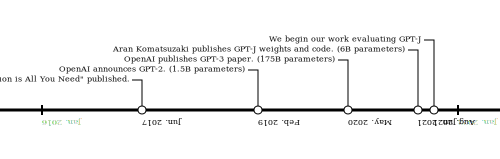
\includegraphics[scale=0.67]{timeline/timeline}}
    \caption[Timeline]{Timeline of Major Transformer-based NLP Models}
\end{figure}
\begin{enumerate}
    \item (Jun. 2017) ``Attention Is All You Need" \cite{Vaswani2017} Was a groundbreaking paper introducing the Transformer network. Transformers became the foundation for the next 5+ years of NLP (Natural Language Processing) research.
    \item (Feb. 2019) OpenAI releases GPT-2, a quantum-leap forward in general NLP tasks. GPT-2 was trained in an un-supervised fashion on 40GB of internet text and has 1.5B parameters. GPT-2 could perform perform rudimentary reading comprehension, machine translation, question answering, and summarization—all without task-specific training.
    \item (May. 2020) OpenAI announces GPT-3\cite{Brown2020} with 100x the parameters of GPT-2 and 10x the parameters of any previous work. GPT-3 had 1000x the dataset size with about 45TB of training text. GPT-3 set a new benchmark in NLP with never-before seen performance and the ability do "few shot learning" where new language tasks could be learned with just a few training examples.
    \item (Jun. 2021) Aran Komatsuzaki and Ben Wang with help from EleutherAI release GPT-J \cite{mesh-transformer-jax}, the first open-source, large-scale, pre-trained transformer based NLP model. With over 6B parameters and trained on 825GB of text, GPT-J provided performance better than GPT-2, and similar to GPT-3. For the first time, the public had unfettered access to enterprise-sized NLP models previously reserved for big companies and cutting-edge researchers.
    \item (Aug. 2021) We begin our research with GPT-J.
\end{enumerate}
\subsection{Transformer Language Model Explained}
\subsubsection{Structure}
The transformer language model has three major steps:
\begin{itemize}
    \item Embedding: This tokenizes the input, converting text into a sequence of integers. Then it embeds the integers into a high-dimensional vector space. This vector representation ideally contains semantic information about the input token.
    \item Self-Attention: The embeddings are then passed through a self-attention layer which looks at the entire input and includes information about context from past tokens. This is a powerful mechanism that allows the model to learn to focus on the most important parts of the input sequence when deciding what to predict.
    \item Feed-Forward: Finally, the output of the self-attention mechanism is passed through a feed-forward network which, using softmax, outputs a probability distribution over the vocabulary. This distribution is then used to generate a prediction of the next token.
\end{itemize}
Together, the self-attention mechanism and the feed-forward network are called a transformer block \cite{yt}. Multiple layers of the transformer block are then stacked together to form a deep network. See figure \ref{fig:transformer}. In general, the deeper the network, the more context and understanding can be stored in the model \cite{yt}.

\begin{figure}[h]
    \centering
    \includegraphics[width=0.45\textwidth]{transformer.png}
    \caption{Data flow of a transformer language model \cite{yt}. Input text is ``The Shawshank". After being de-embedded, the final token should be ``Redemption".}
    \label{fig:transformer}
\end{figure}

\subsection{Relevance \& Novelty of Our Approach}
By our estimation, the vast majority of previous works involving sentiment analysis used a pre-processing step to extract sentiment from the news and then embedded those features into a time-series dataset. News sources were often limited to headlines, tweets and small snippets because of the memory limitations of RNN sentiment classifiers. With the introduction of large transformer networks \cite{Vaswani2017}, capable of processing large amounts of text like OpenAi's GPT-3 \cite{Brown2020} or Wang \& Komatsuzaki's GPT-J \cite{gpt-j}, we believe a new class of trading network can be created. Readily available implementations of GPT-J allow for inputs with up to 2048 input tokens or words. Our method will encode the current world state in a large text input which combines sentiment, real-world facts, and stock price data into a single input.

\section{Preliminary Study}
Our study was broken over two semesters, the first focused on developing a small-scale proof of concept test using the GPT-J-6B weights, and the second focused on developing a larger-scale test using our own fine-tuned weights. We refer to the first semester's small scale work as the \emph{preliminary study} and the second semester's larger scale work as the \emph{main study}.

\subsection{Testing \& Evaluation Methodology}

\subsubsection{Media Release Correlations} \label{math}
To measure the correlation between the release of a media item such as an SEC filing or news story, we will use the standard event study method as detailed in \cite{Neuhierl2010}. This method uses abnormal returns in a given period to calculate the effect of a certain event on a stock's price. Abnormal return for a given day is defined as 
\begin{equation}
    AR_{i,t}=R_{i,t}-(\alpha_i+\beta_i R_{m,t})
\end{equation}
for a firm $i$ at time $t$ where $\alpha_i$ and $\beta_i$ represent the relationship between a given stock and its reference market. And where $R_{m,t}$ is the return of the actual reference market. This method uses the historical relationship of a stock to its reference market to estimate normal returns. Abnormal returns are therefore the difference between the actual return of the stock and the normal return of the stock. 

We can then take large sample of media release events of the same type and calculate the average abnormal return as follows:
\begin{equation}
    AAR= \frac{1}{N} \sum\limits_{i=1}^{N}AR_{i,t}
\end{equation}

Finally, we can measure the total impact of the event over a given period of time by using cumulative abnormal return:
\begin{equation}
    CAR(t_1,t_2)=\sum\limits_{t=t_1}^{t_2} AR_{i,t} 
\end{equation}
where $t_1$ and $t_2$ are the start and end dates of the event window.

Because we are limited in the granularity of data we have access to and can easily process, our research will focus on day-by-day events, returns, and correlations.

\subsubsection{GPT-J Model prediction accuracy}
To evaluate the accuracy of our model given different input data, we will use two metrics. First is a simple ratio of well-formed, parseable outputs to malformed outputs. This first metric we refer to as format-correctness. 
\begin{equation}
    F_c=\frac{N_{parseable}}{N_{malformed}}
\end{equation}
The second metric is a simple ratio of the actual stock price to the predicted stock price. This second metric we refer to as price-accuracy.
\begin{equation}
    P_a=\left|\frac{P_{actual}}{P_{predicted}}\right|
\end{equation}
We will use the price accuracy metric as our loss function in fine-tune training of GPT-J. The format-correctness metric will be used to evaluate the reliability and robustness of our prompt. We may experiment with using the format-correctness metric as a weighted portion of our loss function.
\section{Preliminary Study Implementation}
\subsection{Data Gathering} 
\subsubsection{News Data}
Using the freely available New York Times Archive API {Citation Needed}. We downloaded the associated metadata for each New York Times article from January 2006 through October 2022. This subset of the New York Times archive consists of 1,446,289 articles. We then filtered the articles based on the keywords associated with the article, to get articles relevant to a company in our list of top 50 U.S. companies. Our resulting dataset contains 23,428 unique articles from the Times. We have included a table of the top 50 U.S. companies and their associated ticker symbols in Table \ref{table:stockSources} in Appendix \ref{top50}.

\subsection{Stock Data Gathering}
The next step was to collect a dataset of historical stock prices that can be correlated with the news articles at our disposal. Using the Alpaca Data API v2 \cite{alpacadataapi}, we downloaded the historical stock prices for our top 50 U.S. companies. 
\subsection{Data Preprocessing}
Using the Alpaca API, we were limited to 5 years of past data. This means we must filter our news dataset to start in November of 2016. We were then able to attach stock data with 8,053 news articles over 1,222 weeks (see Figure \ref{fig:eventsPerYear}).
\begin{figure}[h]
    \centering
    \includegraphics[width=0.45\textwidth]{eventsPerYear.png}
    \caption{Number of Events/Year}
    \label{fig:eventsPerYear}
\end{figure}

The dataset was naturally skewed to a certain few companies like Facebook, Netflix, and Apple which account for over 45\% of the news articles in our event dataset despite them only being 3/50 companies or 6\% of the companies included in our news search (see Figure \ref{fig:eventsPerCompany}). 

\begin{figure}[ht]
    \centering
    \includegraphics[width=0.45\textwidth]{eventsPerCompany.png}
    \caption{Number of Events/Company (Top 10)}
    \label{fig:eventsPerCompany}
\end{figure}
\section{Preliminary Study Results}
\subsection{Event Study}
\subsubsection{Standard Methodology}
Our event study had the goal of investigating if the news releases in our dataset were correlated with abnormal returns in stock price. We use the event study methodology as described above in section \ref{math} for each stock in our dataset. Figure \ref{fig:expected} shows the expected return of Facebook compared to its actual return and reference index. Averaging over all the stocks in our dataset, the event study methodology showed that the events in our dataset were not correlated with abnormal returns in stock price.
\begin{figure}[ht]
    \centering
    \includegraphics[width=0.45\textwidth]{FBExpectedValues.png}
    \caption{Facebook: Actual vs. Expected Return}
    \label{fig:expected}
\end{figure} 
\subsubsection{Simple Correlation Test}
To confirm our suspicions that our event data did not correlate with price movements, we ran a simple correlation test on the frequency of news releases for a given company vs. the absolute acceleration of its stock price. Figure \ref{fig:acceleartion} gives an example of this data on Microsoft. The average correlation coefficient over all stocks is 0.035, which means that there is no significant correlation between the news releases and the stock price in our dataset.
\begin{figure}[ht]
    \centering
    \includegraphics[width=0.45\textwidth]{MSFTevents.png}
    \caption{Abs. Acceleration of MSFT vs. News Releases}
    \label{fig:acceleartion}
\end{figure}
\subsection{Inference}
Running inference on models of this scale requires large amounts of parallel compute. With the limited resources of this study, renting Google TPU time to set up our own training and inference environment was intractable. Instead, we used a cloud service called HuggingFace. HuggingFace provides APIs to interface with pre-trained neural models. However, even this service is expensive, so we were unable to perform fine-tune testing. We were also limited to only performing inference on a small subset of our dataset: about 4,000 events.
\subsubsection{Format-Correctness Metric}
Surprisingly, GPT-J was always able to return a parseable output given our test prompt. We have included a sample prompt and response in Appendix \ref{Examples}. We believe that adding a ``\$'' to the end of the prompt made GPT-J more likely to return a parseable output.
\subsubsection{Price-Accuracy Metric}
Our limited inference method was unable to predict stock prices with any accuracy. In our dataset, a simple linear regression over the last week of stock prices was able to generate a prediction of the next day's price 52\% of the time. By comparison, the GPT-J model was correct 47.5\% of the time. Both of these numbers are not significantly better from a random guess. 

\section{Main Study}
\subsection{Data Gathering}
We scraped and labelled 140,000 news articles from the web with the distribution of sources as described in Figure \ref{fig:newsSources}. 
\begin{figure}[h]
    \centering
    \includegraphics[width=0.48\textwidth]{domainCounts}
    \caption{Distribution of News Sources}
    \label{fig:newsSources}
\end{figure}
\subsubsection{Labeling Methodology}
To make sure our dataset was as clean as possible, we used the following labeling method and filtering steps on each of the millions of raw webpages we scraped.
\begin{enumerate}
    \item To be sure each webpage was actually an article and not a landing page, directory page or other non-article page, we used the Mozilla Readability library to determine a readability score for each webpage. We then filtered out all webpages with a score less than 90.
    \item Labelling each article was then done by fuzzy matching company names and ticker symbols to the title and body of the article. We used a list of the top 6500 U.S. companies and their associated ticker symbols to label each article. (See Appendix \ref{top50} for a table of the top 50 U.S. companies and their associated ticker symbols.) Articles with no associated ticker symbol were labeled as ``Unknown'' and were removed from the dataset.
    \item Articles with no associated publication date were removed from the dataset, and the remaining articles were then correlated with the closing stock price of their associated ticker symbol on the date of publication or date prior to the publication date.
\end{enumerate}
\subsection{Fine-tuning}
\subsubsection{Compute}
Compute for both fine-tuning and our inference testing was provided by the Google Research TPU Research Cloud. Our application was approved within 3 months. Google provided credits for 5 TPUv2-8, 100 preemptible TPUv2-8, and 5 TPUv3-8 for one month. This generous donation would have been valued \$144,000 had we purchased the TPU time ourselves.
\subsubsection{Training}
Our dataset of 140,000 was split into a 90K training set, a 10K validation set, and a 40K testing set. Training was done on a TPUv3-8 with a batch size of 32 and 1700 steps. Over training, we saw reductions in loss from around 2.0 to 1.1 (see Figure \ref{fig:loss}). We ran validation tests every 500 steps and our validation loss mirrored our training loss.
\begin{figure}[ht]
    \centering
    \includegraphics[width=0.45\textwidth]{loss.png}
    \caption{Fine-tune Training Loss vs. Steps}
    \label{fig:loss}
\end{figure}
\subsection{Main Study Results}
In testing we found that our fine-tuned model performed no better than random at predicting the next day's stock price. Our fine-tuned model had a prediction accuracy of 50.58\% (N=40,000 articles). Similarly, the un-fine-tuned GPT-J-6B weights had a prediction accuracy of 50.63\% (N=40,000 articles). When compared to a small-scale human test, humans outperformed our model by about 5\%. Human testing had a prediction accuracy of 56\% (N=120 articles).

\section{Conclusion}
Using our training and testing testing methods, GPT-J performs no better than random when predicting the direction of price movement based on a news story. Furthermore, fine-tuning the model with 100,000 articles does not improve prediction accuracy. 
\subsection{Future Work \& Improvements}
We suspect that even though we saw a decrease in loss during training, that this loss only represents the network learning our prompt format. The following steps may improve our technique:
\begin{itemize}
    \item Including more data sources (news, and other) to increase the number of events we can analyze.
    \item Varying prompt format.
    \item More carefully labelled data to reduce noise in the dataset.
    \item Manipulating the loss function to pay more attention to the stock price.
    \item Increasing the size of our training dataset.
    \item Live-training to build a more accurate world model.
\end{itemize}
% \newpage
\begin{singlespace}
	\setstretch{0.9}

\bibliographystyle{IEEEtran}
\bibliography{./paper.bib}
\onecolumn
\begin{Center}
\appendix
\subsection{Top 50 U.S. Companies (November, 2021)}
\label{top50}
\begin{table}[H]
    \caption{Stock Sources}
    \centering
\begin{tabular}{|l|l|}
    \hline
    \textbf{Company} & \textbf{Ticker} \\
    \hline
    Apple & AAPL \\
    Microsoft & MSFT \\
    Alphabet & GOOG \\
    Amazon & AMZN \\
    Facebook & FB \\
    Tesla & TSLA \\
    Berkshire Hathaway & BRK.A \\
    Nvidia & NVDA \\
    JP Morgan & JPM \\
    Visa & V \\
    JOHNSON \& JOHNSON & JNJ \\
    United Health & UNH \\
    Walmart & WMT \\
    Bank of America & BAC \\
    Home Depot & HD \\
    Mastercard & MA \\
    PROCTER \& GAMBLE & PG \\
    Disney & DIS \\
    Adobe & ADBE \\
    Salesforce & CRM \\
    Netflix & NFLX \\
    Exxon & XOM \\
    Oracle & ORCL \\
    Nike & NKE \\
    Comcast & CMCSA \\
    Coca-Cola & KO \\
    Cisco & CSCO \\
    Pfizer & PFE \\
    Fisher Scientific & TMO \\
    Accenture & ACN \\
    Eli Lilly & LLY \\
    Intel & INTC \\
    Pepsi & PEP \\
    Verizon & VZ \\
    Danaher & DHR \\
    Chevron & CVX \\
    Abbott Laboratories & ABT \\
    Broadcom & AVGO \\
    Costco & COST \\
    Merck & MRK \\
    Wells Fargo & WFC \\
    Abbvie & ABBV \\
    Morgan Stanley & MS \\
    AT\&T & T \\
    McDonald's & MCD \\
    Texas Instruments & TXN \\
    Medtronic & MDT \\
    UPS & UPS \\
    Nextera & NEE \\
    \hline
\end{tabular}
\label{table:stockSources}
\end{table}

\subsection{Example Inference Prompt and Response}
\label{Examples}
\begin{lstlisting}[language=json,firstnumber=1]
{
	"q": "On March 01, 2018, the New York times published the following article regarding Walmart(Ticker: WMT) from their Business news desk. Headline: Walmart to Raise Age to Buy Guns and Ammunition to 21. Lead paragraph: Walmart, the largest retailer in the United States, said Wednesday evening that it would stop selling guns and ammunition to anyone under 21 years of age and remove from its stores all toys and airsoft rifles that resemble assault-style weapons. When the news of this was released, past stock prices were: $92.77, $92.89, $93.12, $91.52, $90.01, $89.08. After this news was announced, the following day's price was: $",
	"a": "88.77",
	"r": [
		{"generated_text": "89"}
	]
}
\end{lstlisting}
\end{Center}
\end{singlespace}
\end{document}